%%%%%%%%%%%%%%%%%%%%%%%%%%%%%%%%%%%%%%%%%%%%%%%%%%%%%%%%%%%%%%%%%%%%%%%%%%%%%%%%%%%%%%%%%%%%%%%%%%%%%%%
%%													%%
%% 	BAKALÁŘSKÁ PRÁCE -  Database Output Storage Support in PyWPS Framework			%%
%% 				 Jan Pišl							%%
%%													%%
%% pro formátování využita šablona: http://geo3.fsv.cvut.cz/kurzy/mod/resource/view.php?id=775 	%%
%%													%%
%%%%%%%%%%%%%%%%%%%%%%%%%%%%%%%%%%%%%%%%%%%%%%%%%%%%%%%%%%%%%%%%%%%%%%%%%%%%%%%%%%%%%%%%%%%%%%%%%%%%%%% 

\documentclass[%
  12pt,         			% Velikost základního písma je 12 bodů
  a4paper,      			% Formát papíru je A4
  oneside,       			% Oboustranný tisk
  pdftex,				    % překlad bude proveden programem 'pdftex' do PDF
%%%  draft
]{report}       			% Dokument třídy 'zpráva'
%

\newcommand{\Fbox}[1]{\fbox{\strut#1}}

\usepackage[czech, english]{babel}	% použití češtiny, angličtiny
\usepackage[utf8]{inputenc}		% Kódování zdrojových souborů je UTF8
\usepackage[dvips]{graphicx}   


\usepackage{forest}

\definecolor{folderbg}{RGB}{160,160,160}
\definecolor{folderborder}{RGB}{160,160,160}

\def\Size{6pt}
\tikzset{
  folder/.pic={
    \filldraw[draw=folderborder,top color=folderbg!50,bottom color=folderbg]
      (-1.05*\Size,0.2\Size+5pt) rectangle ++(.75*\Size,-0.2\Size-5pt);  
    \filldraw[draw=folderborder,top color=folderbg!50,bottom color=folderbg]
      (-1.15*\Size,-\Size) rectangle (1.15*\Size,\Size);
  }
}




\usepackage[square,sort,comma,numbers]{natbib}

\usepackage{caption}
\usepackage{subcaption}
\captionsetup{font=small}
\usepackage{enumitem} 
\setlist{leftmargin=*} % bez odsazení

\makeatletter
\setlength{\@fptop}{0pt}
\setlength{\@fpbot}{0pt plus 1fil}
\makeatletter

\usepackage{color}
\usepackage{transparent}
\usepackage{wrapfig}
\usepackage{float} 
\usepackage{listings}
\usepackage{dirtree}


\usepackage{cmap}           
\usepackage[T1]{fontenc}    

\usepackage{textcomp}
\usepackage[compact]{titlesec}
\usepackage{amsmath}
\addtolength{\jot}{1em} 

\usepackage{chngcntr}
\counterwithout{footnote}{chapter}

\usepackage{acronym}

\usepackage[
    unicode,                
    breaklinks=true,        
    hypertexnames=false,
    colorlinks=true, % true for print version
    citecolor=black,
    filecolor=black,
    linkcolor=black,
    urlcolor=black
]{hyperref}         

\usepackage{url}
\usepackage[export]{adjustbox}
\usepackage{fancyhdr}
%\usepackage{algorithmic}
\usepackage{algorithm}
\usepackage{algcompatible}
\renewcommand{\ALG@name}{Pseudokód}% Update algorithm name
\def\ALG@name{Pseudokód}

\usepackage[
  cvutstyle,          
  bachelor,           
]{thesiscvut}


\newif\ifweb
\ifx\ifHtml\undefined % Mimo HTML.
    \webfalse
\else % V HTML.
    \webtrue
\fi 

\renewcommand{\figurename}{Obrázek}
\def\figurename{Obrázek}

%%%%%%%%%%%%%%%%%%%%%%%%%%%%%%%%%%%%%%%%%%%%%%%%%%%%%%%%%%%%%%%%%
%%%%%%%%%%% Definice informací o dokumentu  %%%%%%%%%%%%%%%%%%%%%
%%%%%%%%%%%%%%%%%%%%%%%%%%%%%%%%%%%%%%%%%%%%%%%%%%%%%%%%%%%%%%%%%

%% Název práce
\nazev{Database Output Storage Support in PyWPS Framework}
{Možnosti integrace databázového úložiště v rámci frameworku PyWPS}

%% Jméno a příjmení autora
\autor{Jan}{Pišl}

%% Jméno a příjmení vedoucího práce včetně titulů
\garant{Ing.~Martin~Landa,~Ph.D.}

%% Označení programu studia
\programstudia{Geodesy and Cartography}{}

%% Označení oboru studia
\oborstudia{Geodesy, Cartography and Geoinformatics}{}

%% Označení ústavu
\ustav{Department of Geomatics}{}

%% Rok obhajoby
\rok{2018}

%Mesic obhajoby
\mesic{February}

%% Místo obhajoby
\misto{Prague}

%% Abstrakt
\abstrakt{The aim of this bachelor thesis is to develop design an extension to the PyWPS framework that would enable output data derived from individual PyWPS processes to be stored in a remote database storage. PyWPS is an implementation of the \zk{OGC} Web Processing Service standard. Currently, output data is saved in a standard file format on the server from which the client can download them it. The integration of a database output storage can make more effective both transfering data to the client
and its further processing and analysis. Like PyWPS, the extension is written in Python. As for the database management system, PostgreSQL and PostGIS were used. PostGIS is an extension that adds support for geographic objects to PostgresSQL. The problem of implementing this extension within the PyWPS source code is, to some extent, also adressed in this thesis.}{Cílem této bakalářské práce je navrhnout rozšíření frameworku PyWPS, jenž by umožnilo využít vzdálené databázové úložiště pro ukládání výstupů jednotlivých procesů. PyWPS je implementace standardu \zk{OGC} Web Processing Service. Výstupní data jsou momentálně ukládána v souborových formátech na výpočetním serveru, odkud si je klient může stáhnout. Integrace databázového úložiště může zefektivnit přesun výstupních dat ke klientovi i jejich následnou správu. Rozšíření je - stejně jako framework PyWPS - napsáno v programovacím jazyce Python. Jako vhodný databázový systém byl zvolen PostgreSQL, respektive jeho nadstavba PostGIS, která přidává podporu pro geografické objekty. Součástí práce je i předběžný návrh implementace tohoto rozšíření do zdrojového kódu PyWPS.} \klicovaslova
{PyWPS, databases, Python, GDAL}
{PyWPS, databáze, Python, GDAL}

%%%%%%%%%%%%%%%%%%%%%%%%%%%%%%%%%%%%%%%%%%%%%%%%%%%%%%%%%%%%%%%%%%%%%%%%

%%%%%%%%%%%%%%%%%%%%%%%%%%%%%%%%%%%%%%%%%%%%%%%%%%%%%%%%%%%%%%%%%%%%%%%%
%% Nastavení polí ve Vlastnostech dokumentu PDF
%%%%%%%%%%%%%%%%%%%%%%%%%%%%%%%%%%%%%%%%%%%%%%%%%%%%%%%%%%%%%%%%%%%%%%%%
\nastavenipdf
%%%%%%%%%%%%%%%%%%%%%%%%%%%%%%%%%%%%%%%%%%%%%%%%%%%%%%%%%%%%%%%%%%%%%%%

%%% Začátek dokumentu
\begin{document}

\catcode`\-=12  % pro vypnuti aktivniho znaku '-' pouzivaneho napr. v \cline 

% aktivace záhlaví
\zahlavi

% předefinování vzhledu záhlaví
\renewcommand{\chaptermark}[1]{%
	\markboth{\MakeUppercase
	{%
	\thechapter.%
	\ #1}}{}}

% Vysázení přebalu práce
%\vytvorobalku

% Vysázení titulní stránky práce
\vytvortitulku

% Vysázení listu zadani
\stranka{}%
	{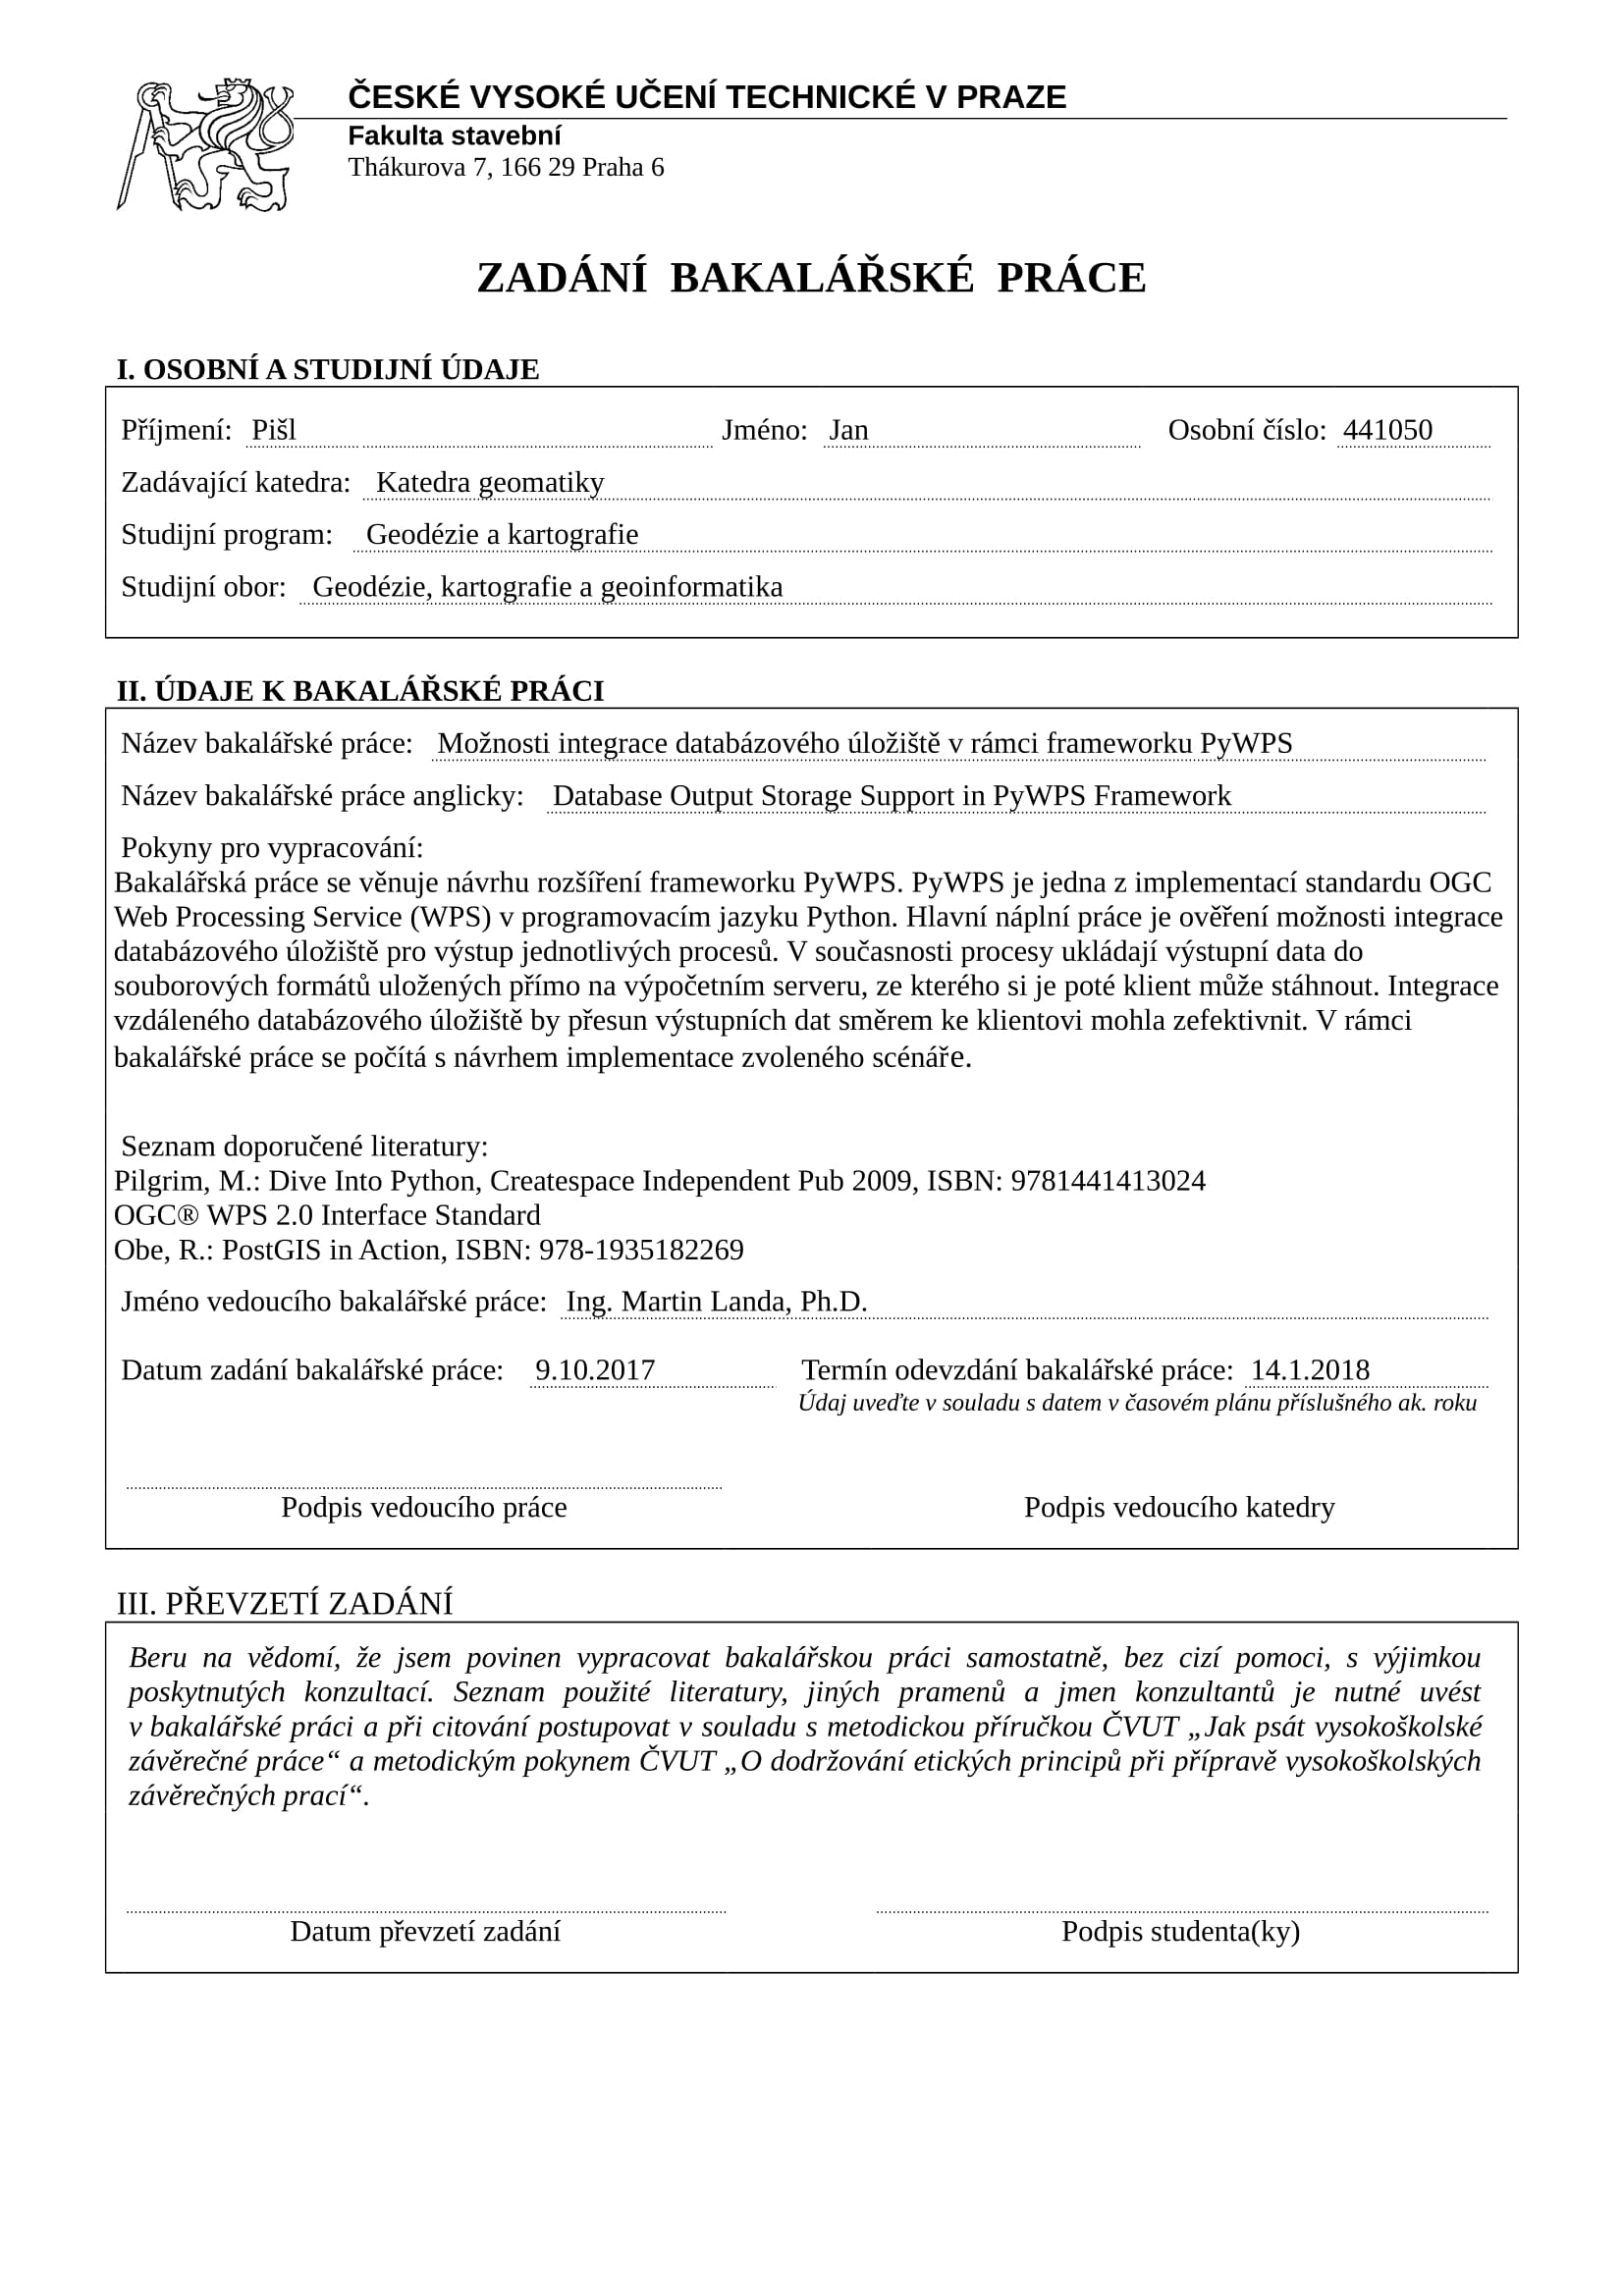
\includegraphics[scale=0.45, center]{./pictures/zadani.jpg}}%\sffamily\Huge\centering\ }%ZDE VLOŽIT LIST ZADÁNÍ}%
	%{\sffamily\centering Z~důvodu správného číslování stránek}
	


% Vysázení stránky s abstraktem
\vytvorabstrakt

% Vysázení prohlaseni o samostatnosti
\vytvorprohlaseni

% Vysázení poděkování
\stranka{%nahore
       }{%uprostred
       }{%dole
       \sffamily
		\begin{flushleft}
		\large
		\MakeUppercase{acknowledgement}
	\end{flushleft}
	\vspace{1em}
		%\noindent
	\par\hspace{2ex}
	{I would like to thank my supervisor, Ing. Martin Landa, PhD., for his guidance, advice and patience.}
}

% Vysázení obsahu
\obsah

% Vysázení seznamu obrázků
%\seznamobrazku

% Vysázení seznamu tabulek
%\seznamtabulek

% jednotlivé kapitoly
\chapter{Introduction}
\label{1-introduction}

Cloud computing - the delivery of on-demand computing resources over a
network (internet or intranet) - is on the rise. Computing resources
may range from relatively simple ones, such as text editors, to very
complex software. They all share the same basic concept – the client
only needs to provide input data, the process itself runs on a server
and then returns the corresponding output data to the client.

Using cloud computing offers a way to gain new capabilities without
investing in new hardware or software. It allows users to perform
complex tasks without having to deal with technical details of the
process. It ensures better collaboration by allowing remote teams to
use the same software. And as all resources are maintained by the
service provider, usually the latest version of the software is
available.

For the above mentioned and other reasons, cloud computing is
frequently used in the field of geoinformation technology and GIS. It
is most useful when it is clear to the client what they need to do and
how to do it and they only lack the tools to perform the task. For
example, the ESRI’s ArcGIS Online platform offers a wide selection of
tools to choose from. These can be “rented” by the client and the task
is then performed on the server. That way, the client gets the desired
data without having to purchase (and learn to use) any desktop GIS
application.

While the benefits of cloud computing are apparent, there is also
another aspect of it that may not get as much attention – the
management of the data produced by such processes. The amount of data
collected and used is increasing rapidly and so is the number of
processes that are being shared on a network. Naturally, the amount of
data derived from such services is growing, too.

Since one of the primary motivation behind cloud computing is to make
the service easy to use for the client, managing output data should
also be carried out by the provider of the service in such a way that
is convenient for the client – it needs to be effective,
well-organized and easy to access.

Relational databases are one way to do so. They are designed and
organized especially for rapid search and retrieval in what can be a
large amount of data. Database-management system (DBMS) is a tool for
managing and interacting with databases.
	
DBMSs have several major advantages over the traditional system where
data is stored in files. Unlike the file management system, there can
be more users accessing the same data concurrently without corrupting
the data. Indexing speeds up the data retrieval operations. There is a
standardized database language to use for queries. There are
mechanisms such as data normalization that can be used to avoid
duplicity of data and save storage space.
	
Being aware of these advantages, the main goal of this thesis is to
design an extension, written in Python, that implements database
storage for output data derived from geoprocessing services run within
the PyWPS framework. They typically produce geographical data, so
appropriate software must be used that is capable of dealing with this
type of data. In this thesis, PostgreSQL is used together with its
spatial database extender PostGIS.

\chapter{Theoretical part}
\label{2-teorie}




\section{Web Processing Services}




\subsection{OGC WPS Implementations}

\begin{itemize}
\item \textbf{PyWPS}
	
  
	
\item \textbf{52°North WPS}
	
  

\item \textbf{ZOO Project}
	
\end{itemize}
  


\subsection{ESRI Web Processing}

\section{Geodatabases}

\begin{itemize}
\item \textbf{PostGIS}
	
\item \textbf{Oracle Spatial and Graph}
%Oracle Spatial and Graph, formerly Oracle Spatial
	
\item \textbf{SpatiaLite}

\item \textbf{ArcSDE Geodatabase (ESRI)}
	
\end{itemize}
\chapter{Technology}
\label{3-technologie}


\section{Python}

\begin{figure}[H] \centering
      
\includegraphics[width=180pt]{./pictures/python-logo-master-v3-TM.png}
      \caption[Python logo]{Python logo (source:
\href{https://www.python.org/static/community_logos/python-logo-master-v3-TM.png}{Python.org})}
      \label{fig:python}
  \end{figure}

  Python is a high-level programming language that fully supports
  object-oriented and structured programming. Developed in the late
  1980s, the first version 0.9.0 was released in 1991. In 2008, Python
  3.0 was released. Currently, the most up-to-date version available
  is 3.6.\cite{diveintopython}

  It was designed as a syntactically simple language, using whitespace
  intendantion instead of brackets and English words rather than
  punctuation. It is a dynamically-typed language, which means it is
  not neccessary to specify a data-type when defining a variable. For
  its simplicity and readability, Python is often considered a good
  first programming language to learn.

  One of the key advantages of Python is its high extensibility. It
  provides large standard libraries and also an extensive number of
  other modules, packages and libraries, so most of the common
  programming tasks are already solved, scripted and made available.



\section{GitHub}

\begin{figure}[H] \centering
      
\includegraphics[width=170pt]{./pictures/github.png}
      \caption[GitHub logo]{GitHub logo (source:
\href{GitHub}{GitHub.com})}
      \label{fig:GitHub}
  \end{figure}

  GitHub is a web-based Git repository hosting service with a
  graphical interface. Git is an open-source version control system
  for tracking changes in text files, typically used for source code
  management.\cite{git} On top of the standard Git functionality,
  GitHub provides a number of its own features, including forking
  (copying a repository), pull requests, or bug tracking. GitHub also
  offers a desktop application.

\section{Geospatial Data Abstraction Library}

\begin{figure}[H] \centering
      
\includegraphics[width=130pt]{./pictures/gdal.png}
      \caption[GDAL logo]{GDAL logo (source:{\cite{gdal}})}
      \label{fig:GDAL}
  \end{figure}

  %% ML: v soucasnosti se jiz pouziva pouze zkratka GDAL, opravil jsem to
  %% ML: dvakrat geospatial ve jedne vete, zkuste prepsat
  Geospatial Data Abstraction Library (GDAL) is the most widely
  used geospatial data acces library for raster and vector geospatial
  data formats. It is released under an X/MIT style Open Source
  license by the Open Source Geospatial Foundation and it is written
  in C++ and C programming languages. As for operating systems, it can
  run under Linux, Solaris, Mac OS X and Microsoft Windows.\cite{gdal}

  The first version was released by Frank Warmerdam in 2000 and the
  last stable version 2.2.3 was released in November
  2017.\cite{gdalrelease}


  %% ML: vypada to, ze chybi OGR ve zkratkach, navrhuji neuvadet jako
  %% zkratku, jasny prepis stejne neexistuje
  The \zk{OGR} library was developed separately but is now a part of
  the \zk{GDAL} source tree. \zk{GDAL} used to work with raster data
  and OGR with vector data. Starting with GDAL 2.0, however, the two
  have been integrated more tightly.

  For its extensive capabilities and comprehensive set of
  functionalities, the GDAL library is widely used by both
  commercial and non-commercial \zk{GIS} projects and programs. The
  list of software programs that uses it includes Google Earth,
  ArcGIS, GRASS \zk{GIS} and many others.\cite{gdalogr}

  %% ML: Nechybi tu PostGIS?
\chapter{Implementation}
\label{4-practical}

\section{Functionality} 

%% ML: use neni moc vhodne slovo, zkuste preformulovat
%% JP: opraveno na consume (to je, myslim, termin, ktery se v tomto kontextu pouziva)
%% ML: muze byt
PyWPS allows to publish and consume geoprocessing services on a
%% ML: zkuste vetu rozdelit (je prilis dlouha, v kratke sekvenci se opakuje 'and')
%% JP: opraveno, snad je to o neco lepsi
%% ML: ano
server. Every process that is to be implemented by PyWPS must be
constructed as a Python class and contain a list of inputs and outputs.
Also, there must be a handler method with two parameters - request and
response. \cite{pywpsprocess} Details on the procedure of creating new
processes can be found in PyWPS documentation.

%% ML: For sending (?)
%% JP: tady bych asi radeji nechal puvodni formulaci, prijde mi prirozenejsi a vyznamove prakticky stejna
%% ML: running at a server?
%% JP: upraveno
%% ML: OK
To send a request to PyWPS, an instance of PyWPS must be running at a server.
%% ML: If it is bych asi uplne vynechal
%% JP: smazano
%% ML: OK
The request is handled and a response is generated and returned
%% ML: file -> document
%% JP: upraveno
%% ML: and -> which ?
%% JP: upraveno {and -> that)
%% ML: OK
to the client. The response has a form of an \zk{XML} document that
contains different elements depending on the type of the request.

When an Execute request is called, a new, temporary folder is created
%% ML: moved -> copied (nejsou odstranena ze zdroje)
%% JP: upraveno
%% ML: OK
in location specified in configuration file and input data is copied
here. While the process is being executed, temporary files may be
generated in this folder. For every process, it must be specified what
the final output is. Once the execution is finished, the output is
copied to a location that is accessible via the web. The temporary
folder, containing input and output data and all the intermediate data
that arose during the execution, is then deleted.

\subsection{Output Data Management}

\subsubsection{Current Options} 

The simplest option of delivering output data is to embed it in the
\zk{XML} response document. Either as plain text, \zk{GML} or, in case
%% ML: encoding scheme
%% JP: upraveno
%% ML: base64 bych ponechal, upraveno
of an image, base64 encoding scheme. This is typically used when the output is
%% ML: where - for PyWPS
%% JP: upraveno, ale myslel jsem, ze to vyplyva z kontextu, cela kapitola se zabyva PyWPS
%% ML: jj
relatively small. For PyWPS, it is also the default option.

%% ML: u obrazku, ktere jste vytvarel uvedte take zdroj (source: author)
%% JP: dopsano
\begin{figure}[H] \centering
  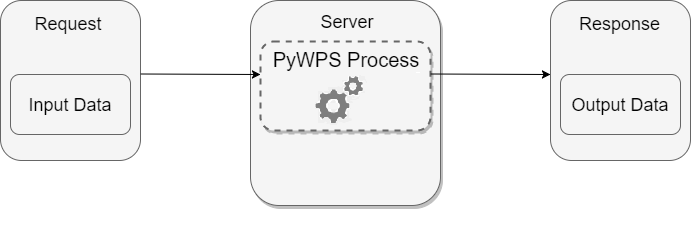
\includegraphics[width=350pt]{./pictures/optionone.png}
  %% ML: zkuste popisek rozsirit, konkretizovat (data odkud kam)
  %% JP: dopsano
      \caption[Delivering output data directly to the client]{Delivering output data directly to the client (source: {author})}
      \label{fig:optionone}
  \end{figure}
  

  If, on the contrary, the output data is large and complex, there is
  another option. The client is only given a reference, a \zk{URL}
  link, from which the data can be downloaded. PyWPS saves the file in
  a folder specified in configuration passed by the service (or in a
  default location). The \zk{URL} is embedded in the \zk{XML}
  response. \cite{pywpsurl}

  %% ML: u obrazku, ktere jste vytvarel uvedte take zdroj (source: author)
  %% JP: dopsano
  %% ML: OK
  
\begin{figure}[H] \centering
  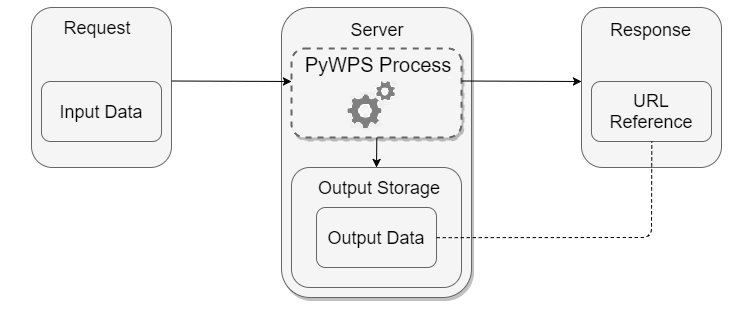
\includegraphics[width=370pt]{./pictures/optiontwo.png}
  %% ML: opet mirne konkretizujte
  %% JP: dopsano
      \caption[Delivering output data via \zk{URL} reference]{Delivering output data via \zk{URL} reference (source: {author})}
      \label{fig:optiontwo}
  \end{figure}

  It is up to the consumer of the process to decide which option to
  choose. For the latter option, the \texttt{"@asReference"} value
  must be set to \texttt{"True"} in the request. \cite{asref} By
  default, it is set to \texttt{"False"}.


\subsubsection{Proposed Extension} 

%% ML: veta nedava moc smysl, prepiste
%% JP: mne smysl dava, konzultoval jsem to s rodilym mluvcim a jemu take. 
%% JP: mate vyhrady z pohledu stylistickeho, nebo vyznamoveho?
%% JP: muzu napsat neco jednoducheho jako "In this thesis, a third
%% JP: option was developed that stores data in a PostGIS database.",
%% JP: ale za sebe nevidim duvod
%% ML: nejak mi tam nesedi: ... the existing two ..., ale pokud jste
%% to konzultoval s rodilym mluvicim, tak to klidne nechte
The aim of this thesis was to develop another variant to add to the
existing two that stores output data in a PostGIS database.

From the point of view of the consumer of a process, it is similar to
the previous option. After the final output has been produced,
connection to the database is established and the output data is
copied there. When the \zk{XML} response is delivered to the client,
%% ML: to neni uplne presne, bude potrebovat pristupove udaje (host
%% name, username, password), viz poznamka nize - jde o jakysi
%% mezikrok 
%% JP: upraveno
%% ML: OK
it contains a reference that points to the location of the data 
within the database. The reference is composed of the name of the database, schema and table. To access the data itself, database login credentials are neccessary.

The current state is not definitive. In the final state, the client
will receive a URL link that references to a \zk{WFS} service. The
\zk{WFS} service itself will access the output data stored in a
database and serve them to the client.

%% ML: doplnte, ze jde o mezikrok (poskytnout referenci na databazi)
%% reseni by se melo doplnit o podporu mapoveho serveru tak, aby
%% klient dostal URL WFS sluzby (ta bude data cist z DB). Pote bude
%% reseni ciste (z pohledu OGC standardu)
%% JP: doplneno
%% ML: v poradku

\begin{figure}[H] \centering
  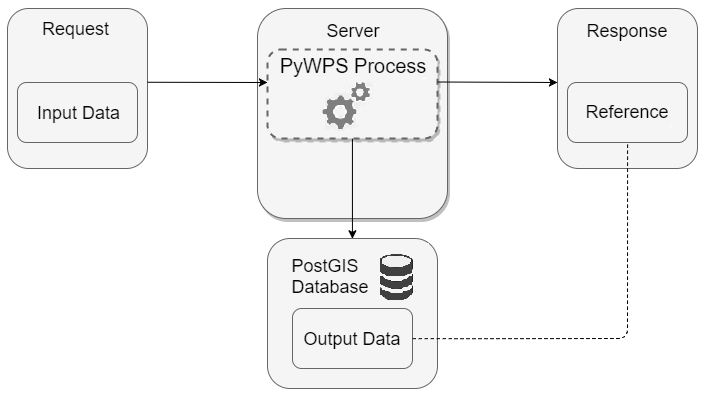
\includegraphics[width=350pt]{./pictures/newoption.png}
    %% ML: opet mirne konkretizujte + zdroj 
    %% JP: doplneno
    %% ML: OK
      \caption[Storing output data in a remote database]{Storing output data in a remote database (source: {author})}
      \label{fig:newoption}
  \end{figure}


To use this functionality as a consumer of a process, it must be implemented in the process by its author. For details on implementation when creating a process, please refer to appendix \ref{appendix}.


\section{Development} 

\subsection{PgStorage class development} 

A new class, \texttt{PgStorage}, has been developed that implements
%% ML: konkretne pro PostGIS (zde by se hodil odkaz do nove kapitoly v
%% technologiich)
%% JP: upraveno, dopsana reference na kapitolu v teorii, kde je PostGIS mezi prost. databazemi
PostGIS storage support. Details on PostGIS can be found in section
 \ref{postgis}. \texttt{PgStorage} is a derived class, inheriting from
\texttt{StorageAbstract} class that is part of PyWPS \zk{API}.
%% part of PyWPS API
%% JP: upraveno
%% ML: OK

%% ML: uvadejte pywps/iout (zpetna lomitka je Windows notace, ktera
%% zde neni podstatna)
%% JP: upraveno
%% ML: misto adresarich mluvte radeji o Python modulech
%% JP: upraveno
%% ML: OK
PgStorage is stored within \texttt{storage.py} in the pywps.inout
module. It consists of several methods that are described below.

\subsubsection{\textunderscore \textunderscore init\textunderscore \textunderscore } 
A constructor, i.e. it gets called automatically when an instance of
the \texttt{PgStorage} class is created.

In this method, the \texttt{get\textunderscore config\textunderscore
  value} function is used that is defined within the PyWPS API. It
accesses the configuration file and retrieves required elements. What
elements are retrieved is specified by the function's two parameters,
section and option.

%% ML: ten popis je mozna prilis detaily, polopatisticky a spatne se
%% cte, muzete zkusit zkratit / zprehlednit
%% JP: trochu preformulovano
%% ML: OK
Correct section (\texttt{db}) is specified and saved to a
variable. The name of the database is extracted from the
configuration file and saved to a variable.

Another variable is defined that serves as a connection string for
connecting to a database. Requisite elements (user name, password and
host server) are retrieved from the configuration file. Finally, an
instance of the \texttt{\textunderscore create\textunderscore schema}
method is created and saved to a variable. See an example of a \texttt{db}
section in section \ref{cfgchanges}.


\subsubsection{\textunderscore create\textunderscore schema} 

%% ML: Opet, ten popis je prilis detailni, nevede to k citelnosti
%% textu, neni to zasadni vytka, klidne nechte, mebo mirne upravte
%% JP: zkraceno
%% ML: OK
First defines a variable \texttt{schema\textunderscore name} as a
random string of specified length that consists of letters and
digits. This is done using Python libraries \texttt{random} and
\texttt{string}.
 
\texttt{Psycopg2} library is used to connect to database
specified by the target variable. A try-except clause is included to raise
an exception if the connection cannot not be established.

Then, when a cursor has been created, an \zk{SQL} query is executed
that generates a new schema if it doesn't exist already. Changes in database are
commited so they persist after connection is aborted, cursor and
connection are closed and the \texttt{schema\textunderscore name}
variable is returned.

\subsubsection{\textunderscore store\textunderscore output}

%% ML: na tomto miste bych spise nez o knihovne OGR mluvil o GDAL
%% (muzete pridat link do technologii, aby byl text lepe provazan)
%% JP: upraveno, pridan link
%% ML: OK
As its name suggests, it handles writing output data to the
database. It benefits from an extensive use of GDAL library. More
information about GDAL can be found in section \ref{gdal}. It has
two input parameters, the name of the file that is to be stored in a
database, and a process identifier.

Thanks to GDAL, the process is fairly simple and straight-forward. The
output file is opened using the file name input parameter and
connection to the database is established. Then, data is copied from
the output file to the database using the OGR \texttt{CopyLayer}
function.

Each of the three above mentioned operations is followed by a simple
condition that checks if the variable storing output of the operation
is not None. If it is, it raises an exception with a corresponding
message.

This method returns the identifier.


\subsubsection{store} 

The store method is defined in the \texttt{StorageAbstract} parent
%% ML: muzete uvest, ze output je v tomto pripade instance tridy ComplexOutput 
%% JP: doplníno
class. Just as in the parent class, it has \texttt{output} as an input
argument. In this case, output is an instance of the \texttt{ComplexOutput} class.

It initializies the \texttt{\textunderscore store\textunderscore
  output} method and passes it name and identifier of the output file.

Then, a string is created that specifies the location of the data and
saved as a variable. It consists of a name of the database, schema and
identifier. This string is then given to the client as an output in
the \zk{XML} response of the process.

There are three parameters returned by the method - the corresponding
value of a DB variable defined within the \texttt{STORE\textunderscore
  %% ML: nazev vystupniho souboru neni v soucasnosti nijak pouzit 
  %% JP: nerozumim. co mam zmenit? metoda prece nazev opravdu vraci, at
  %% uz se pak pouziva, nebo ne.
  %% ML: to byla poznamka na okraj, nic nemente
  TYPE} class, name of the output file and the variable describing the
%% ML: zduraznete ze jde o DB
%% JP: tady take nerozumim
%% ML: posledni promenna vraci "dbname.schema.table" - to neni z vety uplne zrejme
%% JP: doplneno
location of the data that is composed of names of the database, schema and table.
These must be returned as they are required by
the \texttt{get\textunderscore url} method (defined within the
%% ML: presne, viz poznamka vyse
\texttt{ComplexOutput} class).


\subsection{PyWPS source code changes} 

All changes that have been done within the PyWPS source code can be
%% ML: zde uvedte odkaz do prilohy 
examined in a \texttt{diff} folder that is appended to this thesis.
%% ML: diff bude pravdepodobne pouze jeden, vetu muzete vynechat
%% JP: smazano (predpokladal jsem, ze se pro kazdy modul vytvori sam. diff soubor)
%% ML: bude stacit jeden diff se vsim (to je vetsinou standardni postup)

%% ML: tyto zmeny nejsou aktualni!!! v tride Process jiz v soucasnosti
%% zadne zmeny nejsou (pokud se nepletu), text je potreba upravit na
%% zaklade nasi posledni schuzky
%% ML: v kodu jsem odstranil pozustatek zmen (583b5ea), nyni by ve
%% tride Process jiz zadne zmeny byt nemely
%% JP: vychazel jsem z toho jak trida vypadala, kdyz jsem kapitolu psal. ted tedy celou kapitolu mazu
%% ML: OK

%% ML: Output.py neni trida ale Python modul
%% JP: opraveno
\subsubsection{Outputs module}

This module includes three classes that define how outputs are handled
and delivered to the client. Each class deals with one type of output
data - Literal, Complex and BoundingBox.
%% ML: muzete uvest jake tridy tento modul poskytuje (ani ne jejich
%% vycet), ale logicky ramec funkcionalit techto trid (vystupni typy
%% parametru)
%% JP: doplneno
%% ML: OK
Since there is another option being added of storing output data that
returns a reference to the client, \texttt{\textunderscore
  %% ML: uvadite metodu, jake tridy, 
  %% JP: doplneno
  execute\textunderscore xml\textunderscore reference} method in \texttt{ComplexOutput} class had to
be adjusted.

Whether the output data is stored as a file or in a database depends
on value of the \texttt{store\textunderscore type} option in
configuration file. \texttt{store\textunderscore type} is a new
variable within the configuration file that was declared for
this purpose. For details on changes in the configuration file,
refer to section \ref{cfgchanges}. The code block that has been added here
%% ML: toto je nova konfiguracni promenna (to byste mel zminit)
%% JP: pridano
%% ML: OK
first retrieves the value using \texttt{get\textunderscore
  config\textunderscore value}. If it is equal to \texttt{"db"},
\texttt{PgStorage} is chosen to handle output data. In any other case
(the value is different or the option is missing),
\texttt{FileStorage} is used.

%% ML: opet jde o modul, doplnte jake tridy tento modul obsahuje
%% JP: opraveno, doplneno
\subsubsection{Storage module}

\texttt{PgStorage} class has been added that implements the
database storage functionality. For more details on this class,
refer to the section 4.2.1. 

\texttt{FileStorage} is another class defined in this module that inherits 
from \linebreak the \texttt{StorageAbstract} class. As described above, 
it is either this class or  \texttt{PgStorage} that gets called 
when a reference is to be returned within the response document. 
As its name indicates, it saves outputs as files.

There is another class called \texttt{get\_free\_space} within
this module. Its name, too, is self-explanatory - it returns
folder or drive free space.

%% ML: nasledujici dva odstavce jsou duplicitni
%% JP: duplikat odstranen
Also, second option has been added to the class
\texttt{STORE\textunderscore TYPE}.  So, apart from a \texttt{PATH}
variable that implies storing output data as a file, there is also a
\texttt{DB} variable that is used when saving data in a database.

%% ML: testing?
%% JP: myslel jsem to jako odkaz na nazev skriptu (test), ale je to jedno. upraveno
%% ML: za me tez jedno
\subsection{Testing} 

A script has been developed to test whether the process of storing
outputs in a database functions correctly.

For the purpose of this test, three simple processes have been
written. One of them only returns a string, while the other two,
%% ML: text preteka, opravte
%% ML: OK
(\texttt{process\_one\_output} and \linebreak
\texttt{process\textunderscore two\textunderscore outputs}), produce
one and two complex outputs, respectively.

%% ML: zde zminte, ze jde o processy do znacne miry inspirovane
%% procesem z pywps flask demo!
%% JP: mam tam vetu: "They are based on sample processes available for the PyWPS
%% demo service." mam to jeste nejak zduraznovat, nebo to takto staci?
%% ML: staci, asi jsem prehledl
Both \texttt{process\textunderscore one\textunderscore output} and
\texttt{process\textunderscore two\textunderscore outputs} generate
buffers around input features, the latter also calculates centroids
thereof. They are based on sample processes available for the PyWPS
demo service. There is also a \zk{GML} file provided with the demo
service that was used as an input file for this test.

To sucessfully run the test, instance of PyWPS must be running. When
run, the test executes each of the processes and analyzes the
corresponding \zk{XML} response using the ElementTree \zk{XML}
parser. For every process, it returns an identifier of the process
extracted from the \zk{XML} document.

For the two processes that yield complex outputs the test establishes
connection to the database and counts features in the corresponding
table. Then it compares this value to the number of features in the
input file. If these two values differ, it raises an exception.

Similarly, it checks whether the geometry type of the layer in
database is equal to a predefined value (point for centroids, polygon
for buffer). If not, it raises an exception with a corresponding
warning.

When no exception is raised, it indicates that all processes have been
run and all complex outputs have been stored in a database.

%% ML: OGR -> GDAL
%% JP: upraveno
GDAL library is used for creating database connection, counting
features and getting geometry type. Database login credentials are
retrieved from a configuration file using \texttt{get\textunderscore
  config\textunderscore value}. To ensure correct configuration file
is read, another PyWPS built-in function, \texttt{load\textunderscore
  configuration}, is used.
For information on how to download all required data and run the test,
refer to appendix \ref{testing}.

%% ML: pokud bude v priloze ukazka spusteni, tak zde uvedte link
%% JP: doplnil jsem
%% ML: OK

%% ML: podobne by mela byt v priloze ukazka konfigurace (v textu
%% konfiguraci na vice mistech zminujete, doplnte linky do prilohy)
%% JP: v priloze 2 mam ukazku sekce db + store_type=db; staci to tak,
%% JP: nebo jste mel na mysli cely konfiguracni soubor?
%% ML: staci takto
%% JP: nejake linky jsem tam kazdopadne doplnil 

\chapter{Conclusion and future work}
\label{5-conclusion}


The aim of this thesis was to design an extension for the PyWPS framework that would allow output data to be stored in a database rather than in a standard file system. 

Until now, there were only two ways of returning data to the client. It was either embedded in the response directly or, typically if the data was larger or more complex, it remained stored on a server and the response included a reference (a \zk{URL} link) pointing to the location from which the data could be downloaded.

By adding the third option of storing outputs in a remote database, the output data can be transferred, stored and processed more effectively. However, there is a lot of room for improvement and future work. 

Most importantly, current state of the extension provides the client with a string that points to a specific table, schema and database. The client, however, has to access the database by themselves and only then work with the data. 

In the future, the client should be only given a unique \zk{URL} link that points to a running \zk{WFS} or \zk{WMS} service that will be retrievíng data from the database. The client will not even need to be aware where tha data is stored as they will access it easily through a standardized interface. 

The author encountered several other issues during the development. Some of them have been solved, others were out of the scope of this thesis. 

One of the unresolved issues is safety of the database login credentials. At this point, all the data that is neccessary for connecting to and accessing the database (including password) is stored in the configuration file as plain text. Obviously, this is a major safety risk and a better, more secure solution is needed where (at least) the password would not be accessible directly. 

Another problem that may arise if using this extension and that should be addressed in the future is exceeding the capacity of the database if the output data that is being copied to the database is too large. This could be solved by adding another functionality that would establish a connection to the database, check how much space there is available and then compare it to the size of the output file and raise an exception if the capacity was not sufficient.

These and perhaps other improvements are neccessary before the extension can be fully implemented by PyWPS. Due to time constraints, the above mentioned changes will be worked on after this thesis has been submitted. The author plans to cooperate with authors of PyWPS to implement the extension as a pull request to the PyWPS repository.





% Vysázení seznamu zkratek

\begin{seznamzkratek}{ABCDE}
	      
	 \novazkratka{WPS}	
	     {WPS}
	     {Web Processing Service}	  
	     
	\novazkratka{OGC}
	      {OGC}
	      {Open Geospatial Consortium}
	      
	\novazkratka{HTTP}
	      {HTTP}
	      {Hypertext Transfer Protocol}	         
	      
	\novazkratka{XML}
		  {XML}
	      {Extensible Markup Language}

	\novazkratka{DBMS}
	      {DBMS}
	      {Database Management System)}
	         
	  \novazkratka{API}	
	      {API}
	      {Application Programming Interface)}
	           
	  \novazkratka{TIFF}	
	      {TIFF}
	      {Tagged Image File Format}

	  \novazkratka{KML}	
	      {KML}
	      {Keyhole Markup Language}
	      
	  \novazkratka{WKT}	
	      {WKT}
	      {Well-known text}	      
	      
	  \novazkratka{GDAL}	
	      {GDAL}
	      {Geospatial Data Abstraction Library}
	    
	  \novazkratka{GIS}	
	      {GIS}
	      {Geographic Information System}
	     
	  \novazkratka{SQL}	
	      {SQL}
	      {Structured Query Language}
	      
	 
	 
	 
	      
	  \novazkratka{RDBMS}	
	      {RDBMS}
	      {Relational Database Management System}	
	      
	  \novazkratka{WMS}	
	      {WMS}
	      {Web Map Service}	
	      
	   \novazkratka{WFS}	
	      {WFS}
	      {Web Feature Service}     
	      
	   \novazkratka{WCS}	
	      {WCS}
	      {Web Coverage Service}
	      	      
	      	      
	      	      
	   \novazkratka{OSGeo}	
	      {OSGeo}
	      {Open Source Geospatial Foundation} 	  
	     	  
	 	\novazkratka{PFDE}	
	      {PFDE}
	      {Příkon fotonového dávkového ekvivalentu}
	     	  
	 	\novazkratka{PPDE}	
	      {PPDE}
	      {Příkon prostorového dávkového ekvivalentu}
	     	  
	 	\novazkratka{ZHN}	
	      {ZHN}
	      {Zbraně hromadného ničení}
	     	     	  
	 	\novazkratka{JE}	
	      {JE}
	      {Jaderná elektrárna}
	     	  
	 	\novazkratka{MonRaS}	
	      {MonRaS}
	      {Program pro monitorování radiační situace}
	     	  
	 	\novazkratka{SVZ}	
	      {SVZ}
	      {Síť včasného zajištění}
	     	  
	 	\novazkratka{SVZ ARMS}	
	      {SVZ ARMS}
	      {Síť včasného zjištění Armádní radiační monitorovací sítě}
	      
	 	\novazkratka{TDS}	
	      {TDS}
	      {Teledozimetrický systém}	   
	      
	 	\novazkratka{MTF}	
	      {MTF}
	      {the Message Text Format}	         
	      	            	      

\end{seznamzkratek}

% Literatura
\nocite{*}
\def\refname{Bibliography}
\bibliographystyle{mystyle}
\bibliography{literatura}


% Začátek příloh
\def\figurename{Figure}%
\prilohy

% Vysázení seznamu příloh
\seznampriloh

% Vložení souboru s přílohami
%%%%%%%%%%%%%%%%%%%%%%%%%%%%%%%%%%%%%%%%%%%%%%%%%%%%%%%%%%%%%%%%%%%%%%%%%%%%%%%%%%%
%%                 PŘÍLOHA - UŽIVATELSKÁ PŘÍRUČKA                                %%
%%%%%%%%%%%%%%%%%%%%%%%%%%%%%%%%%%%%%%%%%%%%%%%%%%%%%%%%%%%%%%%%%%%%%%%%%%%%%%%%%%%
\chapter{User guide}
\label{user-guide}

The plugin Radiation reconnaissance results uses interpolated radiation
map in raster format as input data. In first step it generates isolines
in preset levels and afterwards converts them into polygons and
simplifies them to fit the limit of total 50 vertices per polygon (in
fact it is 49 as first and last vertex has to have the same coordinates
to close the polygon) for the text message. The output is text file in
NATO APP-11 and ATP-45 compatible format.

\section{Installation}
\label{installation}

Among many ways to install the plugin the easiest one is to install it
from the QGIS plugin repository.

\begin{enumerate}
\item{From \texttt{Plugins} drop down menu select
\texttt{Manage\ and\ Install\ Plugins...}.}

\begin{figure}[H]
    \centering
      \includegraphics[width=200pt]{./pictures/manage_install.jpg}
      \caption{Open dialog of Plugins.}
      \label{fig:manage}
\end{figure}

\item{Go to \texttt{Settings} tab and press \texttt{Add...} button. Write
\url{http://geo.fsv.cvut.cz/geoforall/qgis-plugins.xml} to \texttt{URL}
and press \texttt{OK}. This way you add a path to plugin's home
repository CTU GeoForAll Lab because right now the plugin is not
registered in the official QGIS repository. At this time plugin is
distributed as experimental so if you want to see it you have to tick
the checkbox \texttt{Show\ also\ experimental\ plugins}.}

\begin{figure}[H]
    \centering
      \includegraphics[width=400pt]{./pictures/home_repository.jpg}
      \caption{Add home plugin's repository.}
      \label{fig:repository}
\end{figure}

\item{Go to \texttt{All} or \texttt{Not\ installed} tab and search for
\texttt{Radiation\ \ Reconnaissance\ Results}. Select it and press
\texttt{Install\ plugin} button.}

\begin{figure}[H]
    \centering
      \includegraphics[width=300pt]{./pictures/install_search_plugin.jpg}
      \caption{Search and install the plugin.}
      \label{fig:install}
\end{figure}

\item{The Radiation Reconnaissance Results's icon is now shown in the QGIS
Plugins Toolbar and plugin is ready to use.}

\begin{figure}[H]
    \centering
      \includegraphics[width=200pt]{./pictures/toolbox.jpg}
      \caption{Radiation Reconnaissance Results Plugin on the QGIS toolbar.}
      \label{fig:toolbox}
\end{figure}

\end{enumerate}

\section{Plugin description}

\subsection{GUI}
\label{gui}
The plugin \zk{GUI} is divided into two tabs. The first of them is \texttt{Main}
tab:

\begin{figure}[H]
    \centering
      \includegraphics[width=300pt]{./pictures/main_tab.jpg}
      \caption{The main tab of plugin.}
      \label{fig:main}
\end{figure}

\begin{itemize}
\item{User selects the raster input and chooses appropriate input type (dose
  rate or surface activity). The raster combo box includes available
  layers from the Layer panel or it is possible to upload a raster file
  via button \texttt{Load raster}. By hitting this button, a file
  dialog opens and user can choose desired file (only \zk{GDAL} supported
  files are shown). Pressing \texttt{OK} will insert this path to the
  raster selection. Click on \texttt{Cancel} will interrupt the choosing
  dialog and the raster selection will not be changed.}
\item{Click on a tool button \texttt{...} opens a file dialog where user
  defines the path where the report file will be saved. This file is
  mandatory so \texttt{Solve} button is disabled until path is defined.}
\item{After pressing \texttt{Solve} button, plugin generates simplified
  polygons and saves output file(s) to selected destination(s).}
\end{itemize}

\newpage
The second tab of the plugin is \texttt{Settings} tab:

\begin{figure}[H]
    \centering
      \includegraphics[width=300pt]{./pictures/settings_tab.jpg}
      \caption{The settings tab.}
      \label{fig:settings}
\end{figure}

\begin{itemize}
\item{This tab shows levels used for isolines generation. By default all
  levels available for selected input type are checked but user can
  uncheck particular ones.}
  	\begin{itemize}
		\item{For dose rates the preset levels are 0.1, 1, 5, 10, 50, 100 and 1000 cGy/h.}
		\item{For surface activities the preset levels are 0.01, 1, 10, 100 MBq/m2.}
	\end{itemize}
\item{The last check box allows user to decide if file of simplified
  polygons should be created. This output is optional but by default the
  check box is checked.}
\end{itemize}

\subsection{Input data}
\label{input-data}

\begin{figure}[H]
    \centering
      \includegraphics[width=250pt]{./pictures/input.jpg}
      \caption{Input file.}
      \label{fig:input}
\end{figure}

A raster grid of dose rate or surface activity with a format supported
by \href{http://www.gdal.org/formats_list.html}{GDAL library}. Dose rate
grid units has to be in cGy/h (centiGray/hour = 0.01 Gray/hour), surface
activities in MBq/m2 (megaBecquerel per square meter).

\subsection{Output data}
\label{output-data}

\begin{itemize}
\item{\textbf{Report (mandatory)} 

Structure of the output text report is following:

\texttt{/{[}VALUE{]}{[}UNIT{]}/MGRS:{[}COORDINATE{]}/MGRS:{[}COORDINATE{]}/MGRS:{[}COORDINATE{]}//}
  where:

  \begin{itemize}
  \item{\texttt{VALUE} = dose rate value or surface activity value; decimal separator
    is dot}
  \item{\texttt{UNIT} = used unit in XYH format; where X = C (centi), M (mili), U
    (micro); Y = G (gray), S (sievert); or BQM2 (becquerel per square
    meter)}
  \item{\texttt{COORDINATE} = coordinates in MGRS system, alphanumeric characters}
  \end{itemize}

  All text must be in capital letters. The report must begin with a
  slash, everything between two slashes is called a field. Field 1 can
  contain up to 12 characters. Field 2 can have up to 50 reps (maximum
  50 coordinates), and each field can contain up to 15 characters behind
  the MGRS identifier (eg. accuracy in meters). The last coordinate ends
  with a double slash (indicates the end of a line). Everything between
  the first slash and the double slash is called a line. Individual
  lines must be separated by line break. There must be no space before
  or behind the slash. There is no space between VALUE and UNIT. There
  is no space between \texttt{MGRS:} and the coordinate, the colon must be
  retained.

  The output may contain multiple rows, each being related to another
  level of the measured variable (eg, 3 rows sequentially for 1CGH,
  10CGH and 50CGH).}

\begin{figure}[H]
    \centering
      \includegraphics[width=375pt]{./pictures/vystupni_report.jpg}
      \caption{Output report.}
      \label{fig:report}
\end{figure}
      
\item{\textbf{File of simplified polygons} (optional)

  File of polygons in format Esri Shapefile (\textit{.shp}) is created if check
  box is checked. It is saved in the same directory as input raster
  file.}

\begin{figure}[H]
    \centering
      \includegraphics[width=350pt]{./pictures/vystupni_polygony.jpg}
      \caption{File of simplified polygons.}
      \label{fig:poly}
\end{figure}

\end{itemize}

\chapter{Obsah CD}
\label{cd}


\setlength{\unitlength}{.5mm}
\begin{picture}(250, 220)

  \put(  0, 212){\textbf{.}}

  \put(  1, 200){\line(0, 1){5}}
  \put(  1, 200){\line(1, 0){10} {\textbf{ src}}} 
  \put(150, 200){ zdrojový kód}  

  \put(  1,  190){\line(0, 1){10}}
  \put(  1,  190){\line(1, 0){10} {\textbf{ sample\_data}}}
  \put(150,  190){ testovací data}                     
          
  \put(  1,  180){\line(0, 1){10}}
  \put(  1,  180){\line(1, 0){10} {\textbf{ text}}}
  \put(150,  180){ text práce ve formátu PDF}
      
  \put(  1,  170){\line(0, 1){10}}
  \put(  1,  170){\line(1, 0){10} {\textbf{ zadani}}}
  \put(150,  170){ zadání bakalářské práce}
\end{picture}

% Konec dokumentu
\end{document}
